%%%%%%%%%%%%%%%%%%%%%%%%%%%%%%%%%%%%%%%%%%%%%%%%%%%%%%
%Apêndice A
\hypertarget{estilo:apendice1}{} %% uso para este Guia
%Este apêndice foi criado apenas para indicar como construir um apêndice no estilo, não existia no original da tese.
%%%%%%%%%%%%%%%%%%%%%%%%%%%%%%%%%%%%%%%%%%%%%%%%%%%%%%
\renewcommand{\thechapter}{}%
\chapter{APÊNDICE A - AUTORIZAÇÃO PARA PUBLICAÇÃO}	% trocar A por B na próxima apêndice e etc
\label{apendiceA}	% trocar A por B na próxima apêndice e etc
\renewcommand{\thechapter}{A}%		% trocar A por B na próxima apêndice e etc

Há dois formulários de autorização para publicação, um para publicações de trabalhos acadêmicos e outro para publicações técnico-científicas, neste apêndice encontram-se os modelos dos formulários e suas respectivas instruções de preenchimento. 

\section{Autorização para Publicação de Trabalho Acadêmico - INPE-393}

\label{instr393}

	\begin{figure}[ht]
		\caption{Formulário Autorização para Publicação de Trabalho Acadêmico INPE-393.}
		\vspace{6mm}	% acrescentar o espaçamento vertical apropriado entre o título e a borda superior da figura
		\centering
   		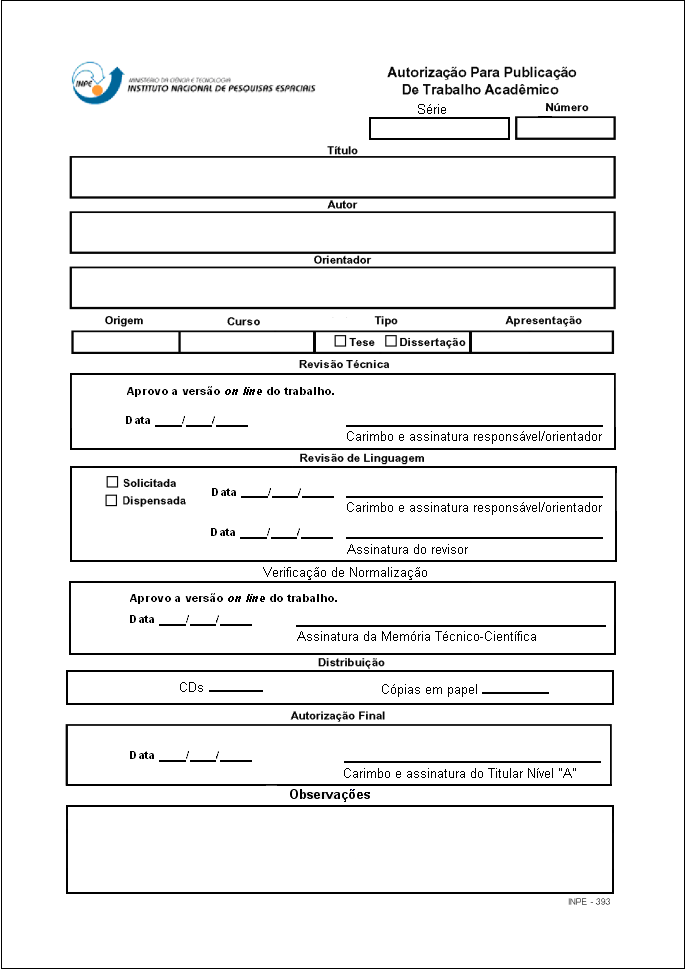
\includegraphics[height=16cm]{./Figuras/form393.png}	   
 		\label{form393}
	\end{figure}


\subsection{Instruções do Formulário INPE-393} 

\begin{enumerate} 

 \item \textbf{série:} com este número o SID identifica as publicações do INPE, composto da sigla da Instituição, número sequencial geral da publicação, sigla e número sequencial do tipo de publicação, exemplo: INPE-14209-TDI/1110;
 
 \item \textbf{número:} será composto da sigla da unidade do SID, mais 4 (quatro) dígitos e do ano em curso. Este número de referência é de controle da unidade emissora. Ex.: SID-0001/2007;

 \item \textbf{título da publicação:} deve ser completo, evitando-se abreviar palavras;

 \item \textbf{nome do autor e do orientador:} estes campos devem ser preenchidos por extenso, da mesma forma em que irão constar da publicação;

 \item \textbf{origem da publicação:} sigla da unidade do servidor (autor da publicação), conforme TQ-001;

 \item \textbf{curso:} sigla do curso, de acordo com a Estrutura de Divisão de Trabalho - EDT do INPE;
 
 \item \textbf{tipo:} assinalar se é tese ou dissertação;

 \item \textbf{apresentação:} colocar a data de aprovação final;

 \item \textbf{revisão técnica:} o responsável designado pela Banca Examinadora para verificação de correções e, na ausência desse, o orientador da tese ou dissertação deve
carimbar, datar e assinar após a versão \emph{on line} do trabalho;

 \item \textbf{revisão de linguagem:} o responsável designado pela Banca Examinadora para verificação de correções, e na ausência deste o orientador deve assinalar a solicitação ou a dispensa da revisão de linguagem e, carimbar, datar e assinar; o revisor deve datar e assinar após a revisão;
 
 \item \textbf{distribuição:} O SID deve informar a quantidade de CD's e de cópias impressas da tese ou dissertação, conforme lista de distribuição;
 
 \item \textbf{verificação de normalização:}  Após a verificação da versão \emph{on line} do trabalho quanto às normas editoriais, o SID deve datar e assinar;
 
 \item \textbf{autorização final:} data e assinatura do Titular de Nível A, conforme TQ-001, a que o Serviço de Pós-Graduação estiver subordinado.
 
 \item \textbf{observações:} para outras informações necessárias. 

\end{enumerate}

\section{Autorização para Publicação - INPE-106}
\begin{figure}[ht!]
	\caption{Formulário Autorização para Publicação de Trabalho Acadêmico INPE-106 folha 1.} 
	\vspace{6mm}	% acrescentar o espaçamento vertical apropriado entre o título e a borda superior da figura
	\centering
	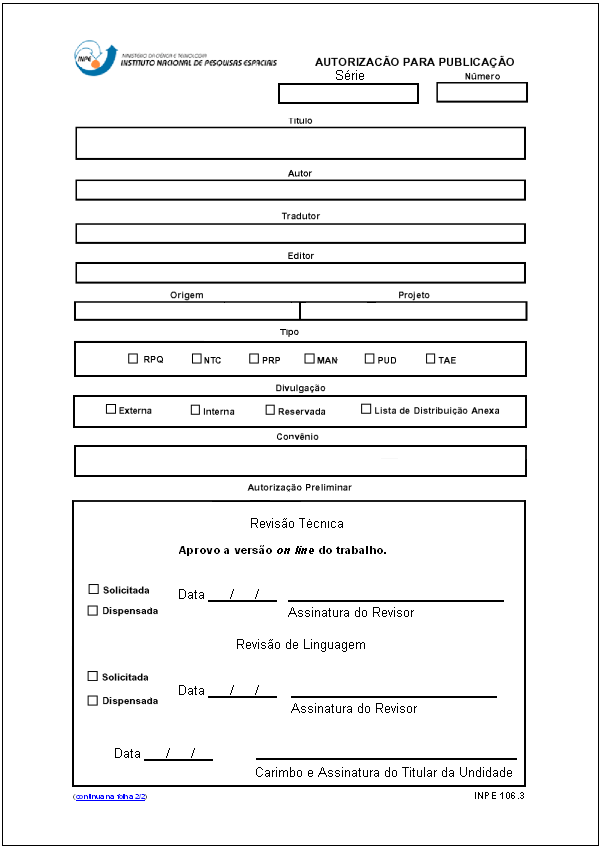
\includegraphics[height=18cm]{./Figuras/form106.png}
	\label{form106}
\end{figure}

\begin{figure}[ht!]
	\caption{Formulário Autorização para Publicação de Trabalho Acadêmico INPE-106 folha 2.} 
	\vspace{6mm}	% acrescentar o espaçamento vertical apropriado entre o título e a borda superior da figura
	\centering
	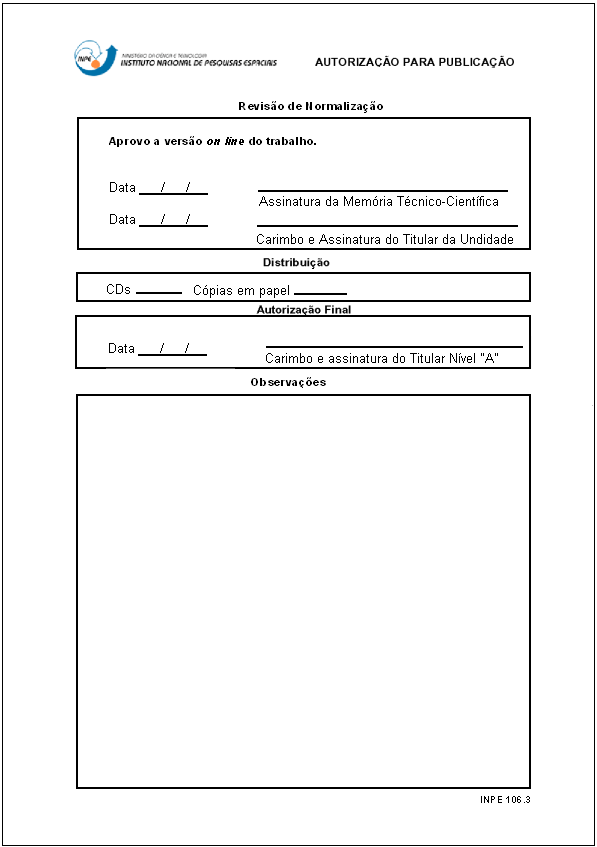
\includegraphics[height=18cm]{./Figuras/form106folha2.png}
	\label{form106a}
\end{figure}

\clearpage
\subsection{Instruções do Formulário INPE-106} 
\label{instr106}


\begin{enumerate}

 \item \textbf{série:} com este número o SID identifica as publicações do INPE, composto da sigla da Instituição, número sequencial geral da publicação, sigla e número sequencial do tipo de publicação, exemplo: INPE-5616-RPQ/671. 
 
 \item \textbf{número:} será composto da sigla da unidade constante da Estrutura Organizacional do INPE (TQ-001), mais 4 (quatro) dígitos e do ano em curso. Este número de referência é de controle da unidade solicitante. Ex: CEA-0001/2007;
 
 \item \textbf{título da publicação:} deve ser completo, evitando-se abreviar palavras;

 \item \textbf{nome do autor, tradutor e editor:}  estes campos devem ser preenchidos por extenso, da mesma forma em que irão constar da publicação;

 \item \textbf{origem da publicação:} sigla da unidade do servidor (autor da publicação), conforme TQ-001;

 \item \textbf{projeto:} sigla do projeto de acordo com a Estrutura de Divisão de Trabalho - EDT do INPE;

 \item \textbf{tipo de publicação:} assinalar o tipo de publicação proposta:

 \begin{enumerate}
  \item{Relátorio de Pesquisa (RPQ)},
  \item{Notas Técnico-Científicas (NTC)},
  \item{Propostas e Relatórios de de Projeto (PRP)},
  \item{Manuais Técnicos (MAN)},
  \item{Publicações Didáticas (PUD)},
  \item{Trabalhos Acadêmicos Externos (TAE)}.
 \end{enumerate}

 \item \textbf{divulgação:} assinalar, de acordo com os critérios de classificação. Se houver Lista de Divulgação, nesta deverá constar os nomes e endereços completos;

 \item \textbf{convênio:} descrever o nome da instituição, quando a publicação for realizada pelo INPE e outra organização, preencher somente para o tipo PRP; 
 
    \item \textbf{autorização preliminar:} data, carimbo e assinatura do Titular da Unidade a que o autor esteja subordinado e, assinatura do revisor que efetuou a revisão técnica aprovando a versão \emph{on line} do trabalho e do revisor que realizou a revisão de linguagem, quando solicitadas; 
    
  \item \textbf{verificação de normalização:} o SID deve datar e assinar após a revisão da adequação às normas editoriais;   
  
  \item \textbf{distribuição:} O SID deve informar a quantidade de CD's e de cópias impressas que deverão ser gravados conforme lista de distribuição;
  
 \item \textbf{autorização final:} data, carimbo e assinatura do Titular de Nível "A", conforme TQ-001, a que o autor da publicação estiver subordinado;
 
 \item \textbf{observações:} para outras informações necessárias, inclusive para descrever as justificativas de uma publicação.
\end{enumerate}